%%%%%%%%%%%%%%%%%%%%%%%%%%%%%%%%%
%
%       EXERCÍCIO
%
%%%%%%%%%%%%%%%%%%%%%%%%%%%%%%%%%

\ifdefstring{\atividade}{prova}{%
    \ifdefstring{\modo}{objetivo}{%
        \renewcommand{\valorquestao}{\ValorQObj\ ponto}
    }{%
        \renewcommand{\valorquestao}{\ValorQDisc\ pontos}
    }%
}%

\begin{exercicioBanco}[\valorquestao]
A curva a seguir representa o gráfico da função \(f(x) = \log_{2}\left(\dfrac{x}{2}\right)\).

\begin{center}
    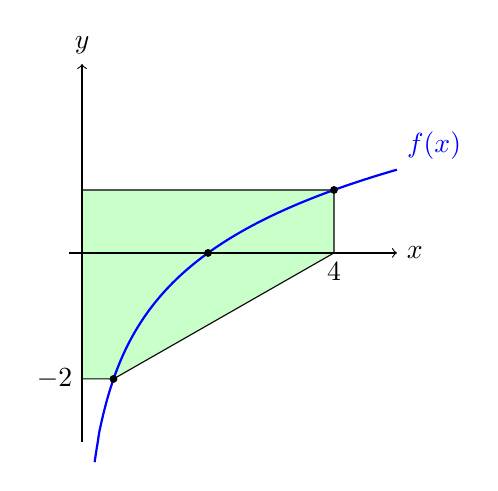
\begin{tikzpicture}[scale=0.8]
        % Região sombreada (aproximando o formato do gráfico)
        \fill[green!30, opacity=0.7]
        (0,-2) -- (0.5,-2) -- plot[domain=0.5:4, samples=200] (\x, {4*\x/7 - 16/7}) -- (4,0) -- (4,1) -- (0,1) -- cycle;   
        
        % Eixos
        \draw[->] (-0.2,0) -- (5,0) node[right] {$x$};
        \draw[->] (0,-3) -- (0,3) node[above] {$y$};
        
        \draw (0,-2) -- (0.5,-2) -- plot[domain=0.5:4, samples=200] (\x, {4*\x/7 - 16/7}) -- (4,0) -- (4,1) -- (0,1) -- cycle;
        
        % Função y = log2(x/2)
        \draw[domain=0.2:5, smooth, samples=200, thick, blue] plot (\x, {ln(\x/2)/ln(2)}) node[above right] {\(f(x)\)};

        % Pontos marcados
        \filldraw (0.5,-2) circle (1.5pt);
        \filldraw (2,0) circle (1.5pt);
        \filldraw (4,1) circle (1.5pt);

        % Rótulos
        \node[left] at (0,-2) {\(-2\)};
        \node[below] at (4,0) {\(4\)};
    \end{tikzpicture}
\end{center}

Calcule a medida da área da região som­breada da figura.
 
% Define as alternativas
\newcommand{\alternativas}{%
    \begin{center}
        \begin{tabularx}{\textwidth}{XXXXX}
            (a) \(\dfrac{17}{2}\). &
            (b) \(\dfrac{21}{5}\). &
            (c) \(8\). &
            (d) \(\dfrac{5}{3}\). &
            (e) \(\dfrac{32}{7}\).
        \end{tabularx}
    \end{center}
}

% Define a resposta correta
\newcommand{\resposta}{A}

% Lógica condicional para exibição
\ifdefstring{\atividade}{lista}{%
    \alternativas
    \vspace{0.5em}
    
    \noindent\textbf{Resposta:} letra \textbf{\resposta}.
}{%
    \ifdefstring{\modo}{objetivo}{%
        \alternativas
    }{%
        % modo = discursiva → não mostra alternativas
    }
}
\end{exercicioBanco}

